\section{Durchführung}
\label{sec:durchführung}
%
Der Versuchsaufbau ist in Abbildung~\ref{fig:aufbau} dargestellt. Die zu untersuchende Kupferprobe (in der Mitte der Abbildung)
befindet sich dabei in einem Zylinder innerhalb des Rezipienten und ist von einem Dewar-Gefäß zur Wärmeisolation umgeben. Damit
verbunden sind die Pt-100 Widerstände zur Temperaturmessung, sowie eine Heizwicklung für die Probe und eine für den Kupferzylinder.
Zur Vorbereitung der Messung wird zunächst der Rezipient über das Ventil zur Vakuumpumpe evakuiert und mit Helium gefüllt. Helium
dient dabei als Medium für den Wärmeaustausch. Das gesamte Innere des Dewar-Gefäßes kann dann durch Befüllen mit flüssigem
Stickstoff auf etwa $\SI{80}{\kelvin}$ abgekühlt werden. Nachdem eine Abkühlung auf diesen Temperaturbereich erfolgt ist, wird der
Rezipient erneut evakuiert und mit der Messung begonnen.
Während der Messung wird die Kupferprobe kontinuierlich elektrisch beheizt. Dabei werden neben dem Widerstand zur
Temperaturermittlung auch Strom, Spannung sowie Dauer des Heizvorganges aufgenommen um die zugeführte Energie ermitteln zu können.
Der Kupferzylinder im Inneren des Rezipienten wird währenddessen über die eigene elektrische Heizung möglichst auf derselben
Temperatur gehalten. Dadurch wird ein Temperaturgefälle vermieden, sodass Wärmeverlust möglichst unterdrückt wird. Es werden so
Messwerte bis zu einer Temperatur von etwa $\SI{300}{\kelvin}$ aufgenommen.

\begin{figure}
    \centering
    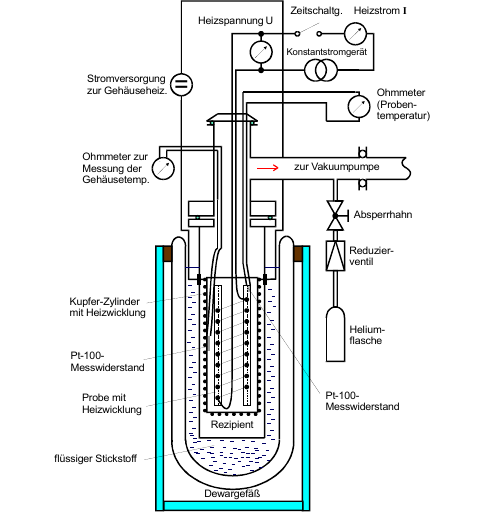
\includegraphics[width=\textwidth]{figures/messapparatur.png}
    \caption{Schematischer Aufbau der verwendeten Messapparatur.\cite{V47}}
    \label{fig:aufbau}
\end{figure}
